\documentclass{article}

%packages included
\usepackage{amsmath}
\usepackage{graphicx}
\usepackage{tabularx}		% lets you choose width of tabular(x) environment
\usepackage{hyperref}
\hypersetup{
    colorlinks=true,
    linkcolor=black,
    filecolor=magenta,
    urlcolor=cyan,
    pdftitle={RoadAI project plan},
    pdfpagemode=FullScreen,
    }
%\usepackage{titlesec}		% see redefinition of \section command
%\uepackagr{minted}		% compile with -shell-escape flag to get syntax highlighting for code blocks (\begin{minted}{<programming lang>} <...>\end{minted}, \inputminted{programming lang}{filename})
%\usepackage{times}		% Times New Roman. \documentclass{article}[12] gives 12 pt. writing.

%custom commands:
\newcommand{\vectorarrow}{\overset{\rightharpoonup}}
%\titleformat{\section}{\normalfont\Large\bfseries}{\thesection}{1em}{}[\hrule]		% redefines \section command. if active along with package "titlesec", will add line under title of each new section

\title{Project Plan - RoadAI}
\author{Berezin, Ilya; Hasle, Viktor R.; Hatland, Ada; Ringkjoeb, Elias}
\date{September $6^{th}$ 2023}

\begin{document}

\begin{titlepage}
\maketitle
\tableofcontents
\end{titlepage}


\section{Overall goal}
In the RoadAI project, we plan to use Multi Agent Reinforcement Learning to reduce emissions coming from
construction machines. Using a data set provided from NORA (Norwegian Artificial Research Consortium) consisting of GPS, vibration and drone data, the goal is to reduce the overall emissions from road construction. We intend to utilize MARL as a techninque to optimize
the trucks idle time as they haul construction materials.

\section{Step-by-step plan}
\begin{enumerate}
  \item Read up on general MARL.\\
  \item Propose a high-level design idea.\\
  \item Make a directory structure for the code, and commit to GitHub.\\
  \item Create environment for MARL in pettingzoo.\\
  \item Implement algorithm for MARL. \\
  \item Evaluate performance of the algorithm.
\end{enumerate}


\section{Meeting plan}
We will be having regular meetings weekly. Depending on the workflow we may decide meet more frequently.
We have also set up a discord channel where we are able to more quickly collaborate.
\section{Methods/tools}
\begin{description}
  \item[PettingZoo] We will be using PettingZoo \href{https://pettingzoo.farama.org}{[1]} to create the environments for the MARL system.
  \item[Rllib] We will be using Rllib \href{https://docs.ray.io/en/latest/rllib/index.html}{[2]} for agent implentation
\end{description}
\section{Timeline}
\begin{figure}[h]
    \begin{center}
        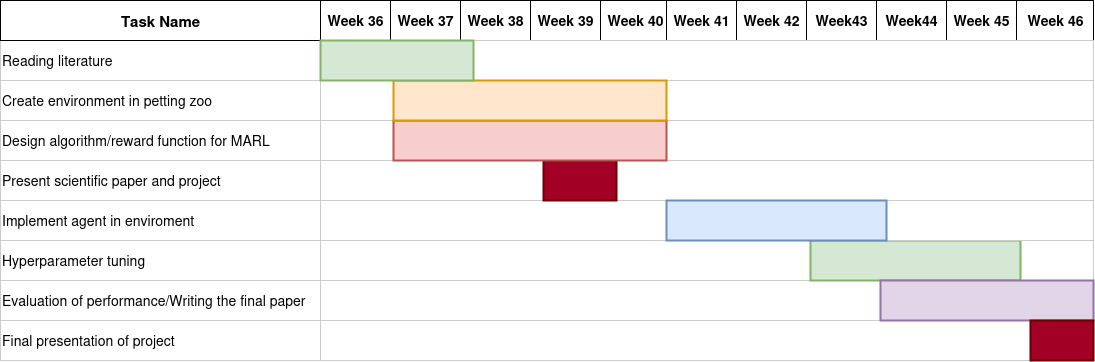
\includegraphics[width=\textwidth]{Timeline.png}
    \end{center}
    \caption{Timeline}
    \label{fig:}
\end{figure}


\section{Responsibilities overview}


\section*{References}
\begin{enumerate}
  \item https://pettingzoo.farama.org
  \item https://docs.ray.io/en/latest/rllib/index.html
\end{enumerate}

\end{document}
